\documentclass[11pt]{article}

% ------------------------------------------------
% Typography
% ------------------------------------------------

\usepackage[T1]{fontenc}
\usepackage[utf8]{inputenc}

\usepackage{XCharter}
\usepackage[charter]{newtxmath}

\usepackage{microtype}

% ------------------------------------------------
% Layout
% ------------------------------------------------

\usepackage[
    left=1.25in,
    right=1.25in,
    top=0.55in,
    bottom=0.80in
]{geometry}

% ------------------------------------------------
% Mathematics
% ------------------------------------------------

\usepackage{amsmath}

% ------------------------------------------------
% Graphics
% ------------------------------------------------

\usepackage{graphicx}
\usepackage{tikz}
\usepackage{xcolor}

% ------------------------------------------------
% Lists
% ------------------------------------------------
% ------------------------------------------------
% Lists
% ------------------------------------------------

\usepackage{enumitem}

\setlist[itemize]{
    leftmargin=1.45em,
    itemsep=3.5pt,
    parsep=0pt,
    topsep=4pt,
    partopsep=0pt
}

% ------------------------------------------------
% Headings
% ------------------------------------------------

\usepackage{titlesec}

\titleformat{\section}
    {\LARGE\bfseries}
    {}
    {0pt}
    {}

\titlespacing*{\section}
    {0pt}
    {0.15em}
    {0.45em}

% ------------------------------------------------
% Hyperlinks
% ------------------------------------------------

\usepackage[hidelinks]{hyperref}

% ------------------------------------------------
% Paragraphs
% ------------------------------------------------

\setlength{\parindent}{0pt}
\setlength{\parskip}{0.25em}

\linespread{1.02}

\pagestyle{empty}

% ==================================================
% DOCUMENT
% ==================================================

\begin{document}











% ==================================================
% SECTION 1
% ==================================================

\section*{\LARGE THE PROBLEM}

{\large
\linespread{1.15}\selectfont

Alice needs \$10,000 cost-of-revision in 24 hours.
How much should she bid given that neither the inclusion time nor the rate at which security will accumulate can be known \emph{ex ante}?

}

\vspace{0.35cm}

\begin{center}

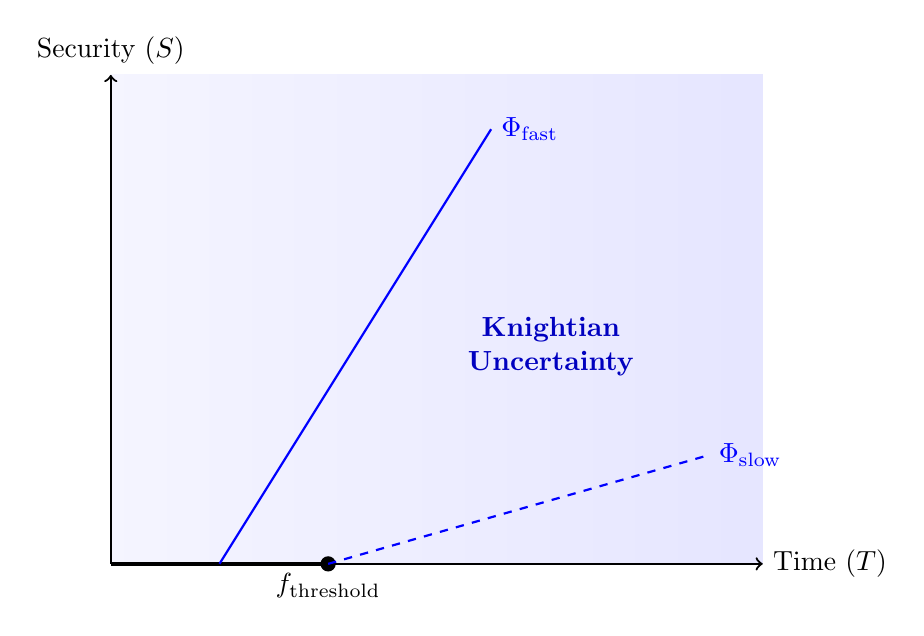
\begin{tikzpicture}[scale=1.38]

    %------------------------------------------------
    % Knightian uncertainty background
    %------------------------------------------------

    \shade[
        left color=blue!4,
        right color=blue!10
    ]
    (0,0) rectangle (6,4.5);

    %------------------------------------------------
    % Axes
    %------------------------------------------------

    \draw[->,thick]
        (0,0)--(6,0)
        node[right]{Time ($T$)};

    \draw[->,thick]
        (0,0)--(0,4.5)
        node[above]{Security ($S$)};

    %------------------------------------------------
    % Threshold
    %------------------------------------------------

    \draw[ultra thick]
        (0,0)--(2,0);

    \fill (2,0) circle (2pt);

    \node[below]
        at (2,0)
        {$f_{\mathrm{threshold}}$};

    %------------------------------------------------
    % Example realizations
    %------------------------------------------------

    \draw[blue,thick]
        (1,0)--(3.5,4)
        node[right]
        {$\Phi_{\mathrm{fast}}$};

    \draw[blue,thick,dashed]
        (2,0)--(5.5,1)
        node[right]
        {$\Phi_{\mathrm{slow}}$};

    %------------------------------------------------
    % Label
    %------------------------------------------------

    \node[
        align=center,
        text=blue!75!black,
        font=\bfseries
    ]
    at (4.05,2.0)
    {Knightian\\Uncertainty};

\end{tikzpicture}

\end{center}

\vspace{0.30cm}

{\large\bfseries
Alice has no truthful bid.
}

\begin{itemize}

\item others bid low? Alice prefers high.

\item others bid high? Alice prefers low.

\end{itemize}

\vspace{0.20cm}

{\large\bfseries
Nor is there a meaningful distribution of types.
}

\begin{itemize}

\item player ``shadow bids'' are always hidden.

\item we cannot reconstruct distributions of types.

\end{itemize}

\vspace{0.20cm}

{\large\bfseries
We have a game under Knightian Uncertainty.
}

\begin{itemize}

\item uncertainty over price aggregation;

\item uncertainty over type distribution;

\item uncertainty over the future;

\item uncertainty over counterparty credibility (Hurwicz).

\end{itemize}


\newpage










% ==================================================
% SECTION 2
% ==================================================

\section*{\LARGE CAN WE ACHIEVE INCENTIVE COMPATIBILITY?}

{\large
\linespread{1.15}\selectfont

Yes. Implementation requires only two assumptions.

}

\vspace{0.35cm}

{\large\bfseries
A. Monotonicity
}


\begin{itemize}
\item Time Monotonicity: increasing the bid weakly increases expected speed of inclusion.
\item Security Monotonicity: increasing the bid weakly increases the slope of the security curve.
\end{itemize}

\vspace{0.30cm}

{\large\bfseries
B. Parallel Games:
}

\begin{itemize}
\item Main Game: bids are public, competition is higher, expected inclusion is faster.
\item Parallel Game: bids are private, competition is lower, expected inclusion is slower.
\end{itemize}

\vspace{0.45cm}

{\large\bfseries
Each player makes two decisions.
}

\begin{itemize}
\item which game to play.
\item which bid to offer.
\end{itemize}

\vspace{0.55cm}






\begin{center}

\begin{tikzpicture}[scale=1.35]

%------------------------------------------------
% Cross
%------------------------------------------------

\draw[thick] (-3.2,0) -- (3.2,0);
\draw[thick] (0,-2.5) -- (0,2.5);

%------------------------------------------------
% Column labels
%------------------------------------------------

\node[font=\large] at (-1.6,2.9) {Lower Fee};
\node[font=\large] at ( 1.6,2.9) {Higher Fee};

%------------------------------------------------
% Row labels
%------------------------------------------------

\node[font=\large] at (-4.2, 1.25) {Main Game};
\node[font=\large] at (-4.2,-1.25) {Parallel Game};

%------------------------------------------------
% Quadrants
%------------------------------------------------

\node[font=\LARGE\bfseries] at (-1.6, 1.25) {$Q_1$};
\node[font=\LARGE\bfseries] at ( 1.6, 1.25) {$Q_2$};

\node[font=\LARGE\bfseries] at (-1.6,-1.25) {$Q_3$};
\node[font=\LARGE\bfseries] at ( 1.6,-1.25) {$Q_4$};

\end{tikzpicture}

\end{center}

\newpage













% ==================================================
% SECTION 3
% ==================================================

\section*{\LARGE WHICH GAME TO PLAY?}

{\large
\linespread{1.15}\selectfont

Our two games differ in only one economically-relevant dimension.

}

\vspace{0.35cm}

{\large\bfseries
The Main Game
}

\begin{itemize}

\item fastest inclusion in expectation;

\item baseline for rational action

\end{itemize}

\vspace{0.35cm}

{\large\bfseries
The Parallel Game
}

\begin{itemize}

\item slower inclusion in expectation;

\item rational only with compensating utility

\end{itemize}

\vspace{0.35cm}


{\large\bfseries
It follows that:
}

\begin{itemize}
\item the two games are substitute methods of coordination
\item one relies on public impersonal incentives, the other on private relational credibility
\item both allow beneficial exchange under the threat of counterparty revision
\item rational choice therefore reveals the marginal rate of substitution between them
\end{itemize}


\newpage
















% ==================================================
% SECTION 4
% ==================================================

\section*{\LARGE EQUILIBRIUM LOGIC}


The role of the mechanism is to enforce \textbf{directional coherence} across games.

\[
\boxed{\text{Bid} \;\longrightarrow\; \text{Speed} \;\longrightarrow\; \text{Security}}
\]


\vspace{0.20cm}

{\normalsize\bfseries
Without this coupling:
}

\begin{itemize}

\item a shift into the parallel game reveals nothing;
\item one opaque utility bundle is preferred to another;
\item there is no identifiable direction of substitution

\end{itemize}

\vspace{0.20cm}

{\normalsize\bfseries
With it:
}

\begin{itemize}

\item one entire class of explanations disappears;
\item preferring the parallel game identifies an unambiguous preference
\item counterparty credibility must be more valuable on the margin;
\item or the game choice itself is irrational.

\end{itemize}

\vspace{0.35cm}


{\normalsize\bfseries
We have a complementary revealed-preference experiment:
}

\begin{itemize}

\item game choice identifies the relevant margin of substitution;
\item bid choice reveals the preferred quantity of security along that margin;
\item yet the mechanism never needs ask players to reveal valuations;
\item as choosing the wrong game is costly in expectation.

\end{itemize}

\vspace{0.35cm}

{\large

The mechanism induces the rational and efficient provision of its baseline
security function relative to an unobservable but strategically-relevant 
substitute (trust in counterparty credibility) that must be optimized 
against for most-efficient provision.


\vspace{0.35cm}

\textbf{Efficient allocation under informational decentralization, contra Hurwicz (1972)}
}

\newpage











% ==================================================
% SECTION 5
% ==================================================

\section*{\LARGE WHY REVELATION EQUIVALENCE FAILS}

{\large
\linespread{1.15}\selectfont

Revelation-equivalent mechanisms cannot preserve the directional coherence
required to implement this equilibrium. Observe:

}

\vspace{0.35cm}

\[
\boxed{
\text{Bid}
\;\longrightarrow\;
\text{Speed}
\;\longrightarrow\;
\text{Security}
}
\]

\[
F \rightarrow T \rightarrow E
\]

\vspace{0.35cm}

Once we add an exogenous informational assumption  (fixed type distribution, common priors, etc) our mapping from bids to security is no longer unique as we introduce an additional determinant of equilibrium $X$.

\vspace{0.35cm}

Our mechanism induces:

\vspace{0.35cm}


\[
F \rightarrow (T,E)
\]

The auxiliary assumption induces:

\[
X \rightarrow E.
\]

\vspace{0.20cm}

Game choice no longer identifies the direction of marginal substitution.

\vspace{0.35cm}

{\large\bfseries
Conclusion.
}

\begin{itemize}

\item efficient allocation under informational decentralization is possible;

\item non-revelation-equivalent mechanisms can preserve directional coherence;

\item a reference mechanism is known that implements this equilibrium

\end{itemize}


\end{document}







